%En este caítulo se presentan los avances que se tienen del sistema en análisis y diseño por cada sprint ...

\section{Estructura del sprint}
En la sección del capítulo se mencionan los componentes que adoptamos del sprint para este proyecto, en esta sección se
describe con mayor detalle cada componente del sprint.\\

\subsection{Planeación del sprint}
En esta sección se detallan el objetivo del sprint, los requerimientos funcionales que debe cubrir, las actividades 
que se deben de realizar y los casos de uso que se deben obtener al finalizar el sprint.

\subsubsection{Requerimientos funcionales}
	Los requerimientos funcionales son descripciones especificas de una función que debe de tener el sistema. Los identificamos 
    por medio de un \textbf{Id} el cual utliza el formato \textbf{RF-MM-XX}, donde:
    \begin{itemize}
        \item \textbf{RF} Es la clave para indicar que es un requerimiento funcional.
        \item \textbf{MM} Es la clave para indicar el modulo al que pertenece.
        \item \textbf{X} Es un número consecutivo: 01, 02, 03, ...
    \end{itemize}

\subsubsection{Casos de uso}
    Los casos de uso son una herramienta usada para representar la interacción entre un actor y el sistema, las cuales siempre 
    tendrán un valor agregado o un propósito para que el actor las realice, son hechos para cubrir con los requerimientos 
    funcionales del sistema.
    En esta sección se van a listar los casos de uso segun el sprint y su diagrama de casos de uso correspondiente.
    Para el diagrama de casos de uso se utiliza la siguiente simbología:
    \begin{itemize}
        \UCpaso Representa al sistema mediante un óvalo.
       \item \UCactor Representa al actor que va a interactuar con el sistema.
       \item Relación $<$- - -$<<extends>>$- - -. Indica que un caso de uso \textbf{puede} ejecutarse a partir de otro.
       \item Relación - - -$<<include>>$- - -$>$. Indica que un caso de uso \textbf{debe} ejecutarse a partir de otro.
   \end{itemize}

   La conexión entre un actor y un caso de uso es por medio de una línea como se muestra en la figura \ref{fig:acUC}.
   

    \begin{figure}[hbtp!]
        \begin{center}
            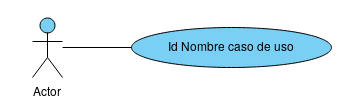
\includegraphics[width=.4\textwidth]{LIT/ActorUC}
        \end{center}
        \caption{Interacción del actor con el caso de uso}
        \label{fig:acUC}
    \end{figure}

    Los casos de uso se encuentran dentro de paquetes (representados por carpetas) indicando así que pertenecen a un mismo módulo 
    como se muestra en la figura \ref{fig:pack}.

    \begin{figure}[hbtp!]
        \begin{center}
            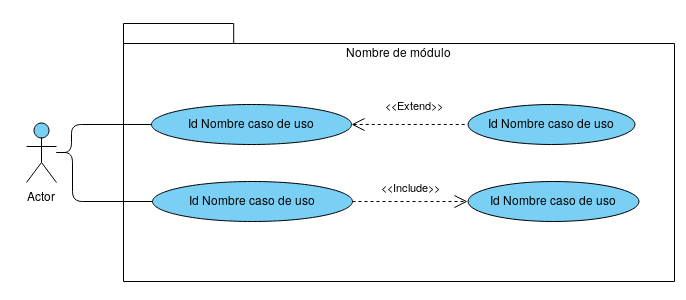
\includegraphics[width=.7\textwidth]{LIT/Paquete}
        \end{center}
        \caption{Un Actor con varios caso de uso dentro de un módulo}
        \label{fig:pack}
    \end{figure}

    En el modelado de los casos de uso se visualizan las funcionalidades del sistema, representadas mediante casos de uso, 
    el modelo de negocio a través de las máquinas de estados, las reglas de negocio y los actores, así mismo, la interacción entre 
    los actores y el sistema a través del menú, interfaces y  mensajes.\\

    A continuación se describen de manera breve a que se refiere cada uno de los puntos mencionados anteriormente.

    \begin{description}
        \item  \textbf{Modelo de estados}: algunas entidades en el sistema  tienen un comportamiento dinámico los que se consideran en el desarrollo del sistema 
        y ameritaban ser modelados a través de una maquina de estados.

        \item  \textbf{Actores del sistema}: se definen los actores identificados como participantes en los procesos del sistema. 
        Estos actores son los encargados de llevar a cabo determinadas tareas dentro de cada proceso es decir, son 
        los responsables de ejecutar el caso de uso.
    
        \item  \textbf{Reglas de negocio}:se describen las reglas de negocio que se utilizan en el sistema las cuales son una condición que se debe satisfacer cuando 
        se realiza cierta actividad de negocio en el sistema.

        \item  \textbf{Caso de uso}:los casos de uso se modelan a partir de dos elementos: un diagrama de casos de uso y la descripción del caso de uso seguida 
        de su interfaz correspondiente.

        \item  \textbf{Mensajes del sistema}: los mensajes se refieren a todos aquellos avisos que el sistema muestra al actor para comunicar la ocurrencia de algún 
        evento tal como un error o una operación exitosa. 
    \end{description}
    

\subsection{Ejecución del sprint}
    En esta sección  se describe el resultado de la ejecución del sprint en la etapa de desarrollo del sistema, incluyendo 
    procesosos, toma de desiciones y obstáculos presentados durante la ejecución del sprint.

\subsection{Revisión y retroalimentación del sprint}
    En esta sección  se describe la evaluación los resultados y aspectos que necesitan ser cambiados.
    En esta fase si se solicitan cambios son realizados o en su caso, si el cambio es muy grande, son intercalarlos en otro
    sprint para no afectar la ejecución del siguiente sprint.
    
    


